\chapter{Pagpapailalim at koordinasyon} \label{ch:subord-coord-tl}

\epigraph{If I were a cinnamon peeler\\
I would ride your bed\\
and leave the yellow bark dust\\
on your pillow.}{Michael Ondaatje, \enquote{The Cinnamon Peeler}}

\begin{tblsframedsymbol}{Mga layunin sa pagkatuto}{bulb}
\begin{itemize}[noitemsep, leftmargin=*]
    \item Maipapaliwanag ang pagkakaiba ng \term{pagpapailalim} (\term{subordination}), na gumagawa ng hirarkiyang pag-asa, at \term{koordinasyon} (\term{coordination}), na nag-uugnay ng mga elementong magkakapantay ang katayuan.
    \item Matutukoy ang \term{sugnay-matrix} (\term{matrix clause}), \term{punong sugnay} (\term{main clause}), at \term{sugnay na nakapailalim} (\term{subordinate clause}) sa masalimuot na pangungusap.
    \item Makikilala ang \term{sugnay-pangnilalaman} (\term{content clause}), \term{sugnay-pahambing} (\term{comparative clause}), at \term{sugnay-relatibo} (\term{relative clause}).
    \item Mauunawaan na ang \term{pangpailalim} (\term{subordinator}) at \term{pangkoordina} (\term{coordinator}) ay mga panandang pangkayarian, hindi mga ulo.
    \item Masusuri ang mga koordinadong kayarian, kabilang ang koordinasyon ng mga parirala at ng mga sugnay.
    \item Magagamit ang mga pagsusuring diagnostiko upang matukoy ang mga relasyong pangkayarian sa masalimuot na pangungusap.
    \item Makikita kung paano nagtutulungan ang pagpapailalim at koordinasyon sa pagbuo ng kohesyon sa teksto.
    \item Mauunawaan ang halagang pedagogiko ng mga kayariang ito sa paglinang ng kamalayang sintaktiko.
\end{itemize}
\end{tblsframedsymbol}

\section{Panimula}

Hindi lamang mga hiwa-hiwalay na ideya ang naipapahayag ng wika; naipapahayag din nito ang mga relasyon sa pagitan ng mga ideya. Dalawang pangunahing paraan nito ang \term{pagpapailalim} (\term{subordination}) at \term{koordinasyon} (\term{coordination}). Magkaiba ang gawain nila. Ang pagpapailalim ay lumilikha ng hirarkiya ng pag-asa. Ang koordinasyon ay nag-uugnay ng mga elementong may pantay na katayuan.

Tingnan ang tatlong paraan ng pag-uugnay ng parehong batayang ideya.

\ea \label{ex:intro-tl}
    \ea \gll Kim left. Pat came.\\
        Kim umalis-PST Pat dumating-PST\\
    \glt \trans{Umalis si Kim. Dumating si Pat.} [magkahiwalay]
    \ex \gll The fact {\ob}that Kim left{\cb} enabled Pat's arrival.\\
        DEF katotohanan Sdr Kim umalis-PST nagpahintulot-PST pagdating ni-Pat\\
    \glt \trans{Dahil sa katotohanang umalis si Kim, naging posible ang pagdating ni Pat.} [nakapailalim]
    \ex \gll Kim left and Pat came.\\
        Kim umalis-PST and Pat dumating-PST\\
    \glt \trans{Umalis si Kim at dumating si Pat.} [koordinado]
    \z
\z
Sa (\ref{ex:intro-tl}a), may dalawang malayang pahayag. Sa (b), ang \mention{that Kim left} ay naipasok sa loob ng mas malaking kayarian. Gumaganap ito bilang komplemento sa loob ng simuno. Sa (c), magkapantay ang dalawang sugnay. Ipinapakita silang magkasing-antas at pinag-uugnay lamang ng \mention{and}.

Mahalaga sa gramatika ang kaibahan ng hirarkiya at pagkakapantay. Kapag ipinailalim natin ang isang sugnay sa isa pa, lumilikha tayo ng relasyon ng pag-asa. Ang isang sugnay ay nagsisilbing komplemento o modipikador ng isang elemento sa mas malaking kayarian. Kapag kinokoordina natin ang mga elemento, ipinapakita nating pareho ang kanilang katayuan sa loob ng kayarian, kahit maaaring magkaiba sila sa ibang bagay.

Iilan lamang ang mga kasangkapang ginagamit sa dalawang relasyong ito. Sa relasyong may pag-asa, ginagamit ang mga salitang gaya ng \mention{that} at \mention{whether}; sa relasyong may pagkakapantay, ginagamit ang \mention{and}, \mention{or}, at \mention{but}. Ngunit sa pamamagitan ng maliliit na salitang ito nakakagawa tayo ng masalimuot na kahulugan mula sa payak na bahagi, naipapakita natin kung paano magkakaugnay ang mga ideya, at nagagabayan natin ang mambabasa sa mahabang takbo ng pangangatwiran. Hindi sila mga ulo; minamarkahan nila ang relasyong gramatikal.

Sa kabanatang ito, titingnan natin kung paano gumagana ang dalawang sistemang ito nang hiwalay at magkasama. Titingnan natin kung paano ipinapasok ng pagpapailalim ang isang ideya sa loob ng isa pa upang makabuo ng mga patong ng kahulugan. Titingnan din natin kung paano nakagagawa ang koordinasyon ng masalimuot na ideya habang nananatiling simple ang kayarian. Sa huli, makikita natin kung paano sila nagtutulungan upang makapagpahayag ng halos anumang relasyong pangkahulugan.

\section{Pagpapailalim}\label{sec:subordination-tl}

Sa komunikasyon, madalas nating kailangang magpahayag ng masalimuot na relasyon sa pagitan ng mga ideya. Maaaring umasa ang isang ideya sa isa pa; maaaring ipaliwanag o baguhin ng isang ideya ang isa pa. Dito pumapasok ang pagpapailalim. Ang \term{pagpapailalim} ay prosesong gramatikal kung saan ginagawang \term{nakaasang bahagi} (\term{dependent}) ang isang sugnay sa loob ng ibang kayarian.

Ang sugnay na naglalaman ng \term{sugnay na nakapailalim} (\term{subordinate clause}) ay tatawagin nating \term{sugnay-matrix} (\term{matrix clause}). Ang sugnay namang hindi nakapaloob sa anumang matrix ay tatawagin nating \term{punong sugnay} (\term{main clause}). Maaaring maging punong sugnay at matrix nang sabay ang isang sugnay, gaya ng ipinapakita sa sumusunod.

\ea \label{ex:sub-basic-tl}
    \ea \gll Kim left early.\\
        Kim umalis-PST maaga\\
    \glt \trans{Maagang umalis si Kim.} [pangunahin]
    \ex \gll She thinks {[}that Kim left early{]}.\\
        siya iniisip-PRS {[}Sdr Kim umalis-PST maaga{]}\\
    \glt \trans{Iniisip niya na maagang umalis si Kim.} [nakapailalim]
    \ex \gll {[}She thinks that Kim left early{]}.\\
        {[}siya iniisip-PRS Sdr Kim umalis-PST maaga{]}\\
    \glt \trans{Iniisip niya na maagang umalis si Kim.} [pangunahin/matrix]
    \z
\z
Ang (\ref{ex:sub-basic-tl}a) ay payak na punong sugnay. Sa (b), ang parehong sugnay ay naging sugnay na nakapailalim: nakaasa na ito sa loob ng sugnay-matrix sa (c). Ang sugnay-matrix sa (c) ay punong sugnay din.

Maaaring lumawak pa ang padron. Sa (\ref{ex:sub-basic2-tl}), ang sugnay sa (\ref{ex:sub-basic-tl}b) ay mula sa pagiging punong sugnay ay naging nakapailalim, ngunit matrix pa rin ito ng \mention{that Kim left}. Sa madaling sabi, maaaring maging punong sugnay at matrix ang isang sugnay, at maaari rin itong maging sugnay na nakapailalim at matrix.

\ea\label{ex:sub-basic2-tl}
\gll I heard {\ob}that she thinks {\ob}that Kim left early{\cb}{\cb}.\\
    ako narinig-PST Sdr siya iniisip-PRS Sdr Kim umalis-PST maaga\\
\glt \trans{Narinig ko na iniisip niya na maagang umalis si Kim.} [nakapailalim]
\z

Ngunit walang sugnay na maaaring maging \term{punong sugnay} at \term{sugnay na nakapailalim} nang sabay. Relasyonal na termino ang \term{sugnay-matrix} at \term{sugnay na nakapailalim}: sinasabi nila ang posisyon ng isang sugnay kaugnay ng isa pa. Ang \term{punong sugnay}, sa kabilang dako, ay tumutukoy sa isang sintaktikong uri. Hindi laging nananatili ang kayarian ng punong sugnay sa lahat ng uri ng sugnay na nakapailalim.

\subsection{Mga uri ng sugnay na nakapailalim}

May tatlong pangunahing uri ng finite na sugnay na nakapailalim sa Ingles.\footnote{Ibinubukod din ng \textit{CGEL} ang finite at non-finite na sugnay na nakapailalim, at may iba pa itong mga sub-uri. Hindi natin tatalakayin ang mga iyon dito.} Ito ang \term{sugnay-pangnilalaman} (\term{content clause}), \term{sugnay-pahambing} (\term{comparative clause}), at \term{sugnay-relatibo} (\term{relative clause}). Tingnan natin ang mga ito isa-isa.

\ea \label{ex:sub-types-tl}
    \ea \gll I doubt that we ordered enough books.\\
        ako duda-PRS Sdr kami umorder-PST sapat libro-PL\\
    \glt \trans{Duda ako kung umorder kami ng sapat na aklat.} [pangnilalaman]
    \ex \gll More books arrived than we had ordered.\\
        mas-marami libro-PL dumating-PST than kami umorder-PST\\
    \glt \trans{Mas maraming aklat ang dumating kaysa inorder namin.} [pahambing]
    \ex \gll The books that we ordered arrived.\\
        DEF libro-PL Rel kami umorder-PST dumating-PST\\
    \glt \trans{Dumating ang mga aklat na inorder namin.} [relatibo]
    \z
\z
Ang mga sugnay-pangnilalaman ang batayang uri. Wala sa kanila ang mga espesyal na katangiang sintaktiko ng mga sugnay-relatibo o sugnay-pahambing. Ang mga sugnay-relatibo ang paksa ng susunod na kabanata, kaya dito muna natin titingnan ang mga sugnay-pangnilalaman, pagkatapos ang mga sugnay-pahambing.

\subsubsection{Sugnay-pangnilalaman}

May dalawang pangunahing uri ng sugnay-pangnilalaman: deklaratibo at interrogatibo. Tingnan ang (\ref{ex:content-types-tl}).\footnote{Tinatalakay din ng \textit{CGEL} ang exclamative na sugnay-pangnilalaman, ngunit bihira ang mga iyon.}

\ea \label{ex:content-types-tl}
    \ea \gll She said that it was genuine.\\
        siya sinabi-PST Sdr ito naging-PST tunay\\
    \glt \trans{Sinabi niya na tunay iyon.} [deklaratibo]
    \ex \gll She asked whether it was genuine.\\
        siya nagtanong-PST whether ito naging-PST tunay\\
    \glt \trans{Tinanong niya kung tunay iyon.} [batayang tanong]
    \ex \gll She asked what made it genuine.\\
        siya nagtanong-PST what gumawa-PST ito tunay\\
    \glt \trans{Tinanong niya kung ano ang nagpapaging tunay dito.} [nakapokus na tanong]
    \z
\z
Mahalaga ang ginagawa ng \mention{that} at \mention{whether} sa (\ref{ex:content-types-tl}a at b). Ipinapakita nila na nakapailalim ang kani-kanilang sugnay. Dito pumapasok ang isang bago ngunit napakaliit na kategorya: ang \term{pangpailalim} (\term{subordinator}, Sdr). Pangunahing kasapi nito ang \mention{that}, \mention{whether}, at ang \mention{if} kapag nangangahulugang \enquote{whether}, hindi ang kondisyunal na \mention{if}.

Sa Tagalog, maaaring tawaging \enquote{pang-ugnay} ang napakaraming salita, mula sa pangatnig hanggang sa panandang pandiskurso. Mas makitid ang ibig sabihin ng \term{pangpailalim} dito: isang sintaktikong pananda ito, hindi pangkalahatang salita para sa anumang nag-uugnay.

May NP ang noun at VP ang verb, ngunit walang SdrP ang pangpailalim. Hindi ito nagpo-project ng sariling parirala; minamarkahan lamang nito kung paano kaugnay ng mas malaking kayarian ang sugnay. Ipinapakita ang puno sa Figure~\ref{fig:sub-tree-sub-tl}. (Ang mga tatsulok ay nagpapakitang may nakatagong bahagi ng kayarian; tingnan ang Kabanata 6.)

\begin{figure}
    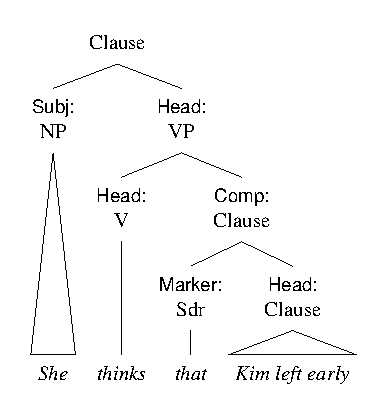
\includegraphics[width=0.55\linewidth]{figures/she thinks that kim left.pdf}
    \caption{Punong sintaktiko na nagpapakita ng pagpapailalim: ang \mention{that Kim left early} ay gumaganap bilang komplemento sa \mention{She thinks that Kim left early}}\label{fig:sub-tree-sub-tl}
\end{figure}

Pansinin na sa nakapailalim na kayarian, lumilitaw ang \mention{that} bilang pananda. Hindi ito nagpo-project ng sarili nitong parirala; minamarkahan lamang nito ang simula ng sugnay na nakapailalim. Ang \term{pananda} (\term{marker}, Mk) ay uri ng nakaasang bahagi na nagpapakita kung paano nakakabit sa mas malaking kayarian ang ulo nito.

Maaaring gumanap sa iba-ibang paraan ang mga sugnay-pangnilalaman sa loob ng mas malaking kayarian.

\ea \label{ex:content-funcs-tl}
    \ea \gll I suspect {\ob}that he left{\cb}.\\
        ako hinala-PRS Sdr siya umalis-PST\\
    \glt \trans{May hinala ako na umalis siya.} [sa loob ng VP]
    \ex \gll The fact {\ob}that he left{\cb} is clear.\\
        DEF katotohanan Sdr siya umalis-PST ay-PRS malinaw\\
    \glt \trans{Malinaw ang katotohanang umalis siya.} [sa loob ng NP]
    \ex \gll I'm glad {\ob}that he left{\cb}.\\
        ako-maging masaya Sdr siya umalis-PST\\
    \glt \trans{Natutuwa ako na umalis siya.} [sa loob ng AdjP]
    \ex \gll We can proceed provided {\ob}that he left{\cb}.\\
        kami maaari-PRS magpatuloy provided Sdr siya umalis-PST\\
    \glt \trans{Maaari tayong magpatuloy kung umalis na siya.} [sa loob ng PP]
    \ex \gll Whether or not he left is unclear.\\
        whether or not siya umalis-PST ay-PRS hindi-malinaw\\
    \glt \trans{Hindi malinaw kung umalis siya o hindi.} [simuno]
    \ex \gll It's unclear whether or not he left.\\
        it-ay hindi-malinaw whether or not siya umalis-PST\\
    \glt \trans{Hindi malinaw kung umalis siya o hindi.} [extraposed na simuno]
    \z
\z

Sa deklaratibong sugnay-pangnilalaman, ang pananda, ibig sabihin ang pangpailalim na \mention{that}, ay maaaring sapilitan, opsiyonal, o hindi pinapayagan depende sa gawain ng sugnay.

\ea\label{ex:marker-need-tl}
    \ea \gll That Kim left surprised no one.\\
        Sdr Kim umalis-PST gumulat-PST walang-isa\\
    \glt \trans{Hindi ikinagulat ng sinuman na umalis si Kim.} [sapilitan]
    \ex \gll I know that Kim left.\\
        ako alam-PRS Sdr Kim umalis-PST\\
    \glt \trans{Alam ko na umalis si Kim.} [opsiyonal]
    \ex \gll *We left before that Kim arrived.\\
        *kami umalis-PST before Sdr Kim dumating-PST\\
    \glt \trans{Inaasahang kahulugan: umalis kami bago dumating si Kim. Sa Ingles, hindi maaaring gamitin dito ang \mention{that}.} [*; hindi tanggap]
\z
\z
Sa mga sugnay na simuno gaya ng (\ref{ex:marker-need-tl}a), laging kailangan ang pananda. Bilang komplemento, karaniwang maaaring magkaroon o mawalan ng pananda ang deklaratibong sugnay, gaya ng (b). Ang malaking eksepsiyon ay kapag gumaganap itong komplemento sa loob ng PP, gaya ng (c).

\label{sec:sub-interrog-tl}

Kawili-wili ang mga interrogatibong sugnay-pangnilalaman dahil iba ang sintaks nila sa pangunahing sugnay na tanong. Ang pangunahing batayang tanong gaya ng \mention{Did she accept?} ay nakikilala sa pagbaligtad ng simuno at auxiliary. Sa nakapailalim na bersiyon, ang pagiging tanong ay minamarkahan ng \mention{whether} o \mention{if}.

\ea batayang sugnay na tanong\label{ex:int-sub-tl}
    \ea \gll Did she accept?\\
        AUX siya tumanggap\\
    \glt \trans{Tinanggap ba niya?} [pangunahin, may baligtad]
    \ex \gll I wonder {\ob}whether she accepted{\cb}.\\
        ako nagtataka-PRS whether siya tumanggap-PST\\
    \glt \trans{Iniisip ko kung tinanggap niya.} [nakapailalim]
    \z
\z
\ea nakapokus na sugnay na tanong
    \ea \gll How did we get here?\\
        how AUX kami nakarating dito\\
    \glt \trans{Paano tayo nakarating dito?} [pangunahin, may baligtad]
    \ex \gll I wonder {\ob}how we got here{\cb}.\\
        ako nagtataka-PRS how kami nakarating-PST dito\\
    \glt \trans{Iniisip ko kung paano tayo nakarating dito.} [nakapailalim]
    \z
\z
Mahirap ito para sa mga nag-aaral ng Ingles. Madalas na hindi nagbabaligtad ang mga baguhan at mali ang nabubuong pangunahing tanong. Kapag natutuhan na ng mas may karanasang mag-aaral ang pagbaligtad, minsan inilalagay nila ito kahit saan at nagkakamali sa nakapailalim na tanong. Kailangan ng mataas na kahusayan bago maging madali ang pagkakaibang ito.

Gayunman, unti-unting humihina ang layo ng kayarian ng pangunahing tanong at nakapailalim na tanong. Dahan-dahang kumakalat ang pagbaligtad. Bihira pa rin sa pagsulat ang interrogatibong sugnay-pangnilalaman na may baligtad, ngunit karaniwan na sa pagsasalita ang mga halimbawa gaya ng (\ref{ex:non-inverted-interrogative-tl}). Baka pagkalipas ng ilang siglo, maging pamantayan sa lahat ng tanong ang pagbaligtad at maging opsiyonal ang mga pananda. Hindi ako maghihintay.

\ea\label{ex:non-inverted-interrogative-tl}
\gll We need a story of {\ob}how did we get here{\cb}.\\
    kami kailangan-PRS a kuwento of how AUX kami nakarating dito\\
\glt \trans{Kailangan natin ng kuwento tungkol sa kung paano tayo nakarating dito.}
\z
Ngunit sa kasalukuyang Ingles, halos laging kailangan ang panandang gaya ng \mention{whether} o \mention{if} sa batayang interrogatibong sugnay-pangnilalaman. Kung wala ito, sa karamihan ng kaso ay hindi ito madaling maihihiwalay sa walang-panang deklaratibong sugnay.

\subsubsection*{Mandative na kayarian}

Isang espesyal na sub-uri ng nakapailalim na kayarian ang \term{mandative na kayarian} (\term{mandative construction}). Lumilitaw ito kasama ng mga panaguring nagpapahayag ng kahilingan, utos, o pangangailangan.

\ea \label{ex:mandative-tl}
    \ea \gll It is essential {\ob}that he be there{\cb}.\\
        it ay-PRS mahalaga Sdr siya be-PLAIN doon\\
    \glt \trans{Mahalagang nandoon siya.} [present subjunctive]
    \ex \gll It is essential {\ob}that he should be there{\cb}.\\
        it ay-PRS mahalaga Sdr siya should be doon\\
    \glt \trans{Mahalaga na dapat nandoon siya.} [should]
    \ex \gll It is essential {\ob}that he is there{\cb}.\\
        it ay-PRS mahalaga Sdr siya be-PRS doon\\
    \glt \trans{Mahalaga na nandoon siya.} [indicative]
    \z
\z
Sa \term{present subjunctive} (\term{present subjunctive}), ginagamit ang plain form ng pandiwa. Hindi ibig sabihin ng \enquote{subjunctive} dito na hindi totoo o counterfactual ang pangungusap. Sa Ingles na \mention{that he be there}, mahalaga ang paggamit ng \mention{be} bilang plain form sa konteksto ng pangangailangan o kahilingan. Ang anyong may \mention{should} ay mas karaniwan, o dating mas karaniwan, sa British English. Mas pinipili ng American English ang present subjunctive. Sa \term{indicative} (\term{indicative}), ginagamit ang ordinaryong anyong may tense.

Makikita rito na kahit sa loob ng sugnay na nakapailalim, maaaring may pinong pagkakaiba ng kahulugan at rehiyonal na hilig. Mula sa pananaw ng pagtuturo, mahalagang sabihin na lumalaganap ang indicative, lalo na sa impormal na konteksto, ngunit pamantayan pa rin sa pormal na pagsulat ang present subjunctive.

\begin{tblsframedsymbol}{Suriin ang pag-unawa: matrix at nakapailalim na sugnay}{test}
Hanapin ang mga relasyong pangkayarian.
\begin{itemize}[noitemsep, leftmargin=*]
    \item Sa \mention{I know that she thinks that he left}, tukuyin ang punong sugnay, mga sugnay-matrix, at mga sugnay na nakapailalim.
    \item Ipaliwanag kung bakit walang pagbaligtad sa \mention{She asked whether he left}, ngunit mayroon sa \mention{Did he leave?}.
    \item Hanapin ang mandative na kayarian: \mention{It's important that he be careful} at \mention{It's important that he is careful}.
\end{itemize}
Kapag nauunawaan ang mga relasyong ito, mas malinaw kung paano nalilikha ang kahulugan mula sa kayariang sintaktiko.
\end{tblsframedsymbol}

\subsection{Sugnay-pahambing}

Ang ikalawang pangunahing uri ng finite na sugnay na nakapailalim ay ang sugnay-pahambing. Kinukumpleto ng sugnay-pahambing ang paghahambing gaya ng nasa (\ref{ex:comparative-intro-tl}).

\ea \label{ex:comparative-intro-tl}
    \ea \gll The ice was thicker than {\ob}we expected{\cb}.\\
        DEF yelo naging-PST mas-makapal than kami umasa-PST\\
    \glt \trans{Mas makapal ang yelo kaysa inaasahan namin.}
    \ex \gll She writes faster than {\ob}she speaks{\cb}.\\
        siya sumulat-PRS mas-mabilis than siya magsalita-PRS\\
    \glt \trans{Mas mabilis siyang sumulat kaysa magsalita.}
    \ex \gll It doesn't cost as much as {\ob}I'd thought{\cb}.\\
        it NEG halaga-PRS as marami as ako-akala-PST\\
    \glt \trans{Hindi ito kasingmahal ng akala ko.}
    \z
\z

Ang katangiang naghihiwalay sa sugnay-pahambing mula sa sugnay-pangnilalaman ay may ellipsis ito. May bahaging naiiwan dahil mababawi ito mula sa konteksto. Sa (\ref{ex:comparative-ellipsis-tl}), ipinapakita ng ... ang bahaging naiiwan.\footnote{Naipakilala na ang gap sa naunang kabanata. Ang gap ay posisyong pangkayarian sa loob ng puno. Sa ellipsis, mababawi ang naiwan sa kahulugan mula sa konteksto, ngunit hindi ito naroon bilang sintaktikong elemento.}

\ea \label{ex:comparative-ellipsis-tl}
    \ea \gll Kim read more books than {\ob}Pat read ...{\cb}.\\
        Kim basa-PST mas-marami libro-PL than Pat basa-PST ...\\
    \glt \trans{Mas maraming aklat ang binasa ni Kim kaysa binasa ni Pat.}
    \ex \gll Kim read more books than {\ob}Pat did ...{\cb}.\\
        Kim basa-PST mas-marami libro-PL than Pat AUX.PST ...\\
    \glt \trans{Mas maraming aklat ang binasa ni Kim kaysa kay Pat.}
    \ex \gll Kim read more books than {\ob}Pat{\cb}.\\
        Kim basa-PST mas-marami libro-PL than Pat\\
    \glt \trans{Mas maraming aklat ang binasa ni Kim kaysa kay Pat.}
    \z
\z

Sa unang dalawang anyo, nakikita ang ellipsis. Sa (b), ginagamit ang VP pro-form na \mention{did} sa halip na ulitin ang \mention{read}. Sa ikatlong anyo (c), hindi komplemento ng sugnay ang \mention{Pat}; NP complement ito. Halos pareho ang batayang kahulugan ng tatlo.

Hindi gaya ng karamihan sa ellipsis, nagiging hindi tanggap ang sugnay-pahambing kapag tahasang binanggit ang naiwan. Halimbawa, hindi sinasabi ang *\mention{Kim read more books than Pat read 20 books} o *\mention{It's not as deep as it is 20 cm wide}. Sentral sa ganitong uri ng sugnay ang ellipsis. Makikita ang kayarian ng sugnay-pahambing sa Figure~\ref{fig:comp-tree-tl}.

\begin{figure}
    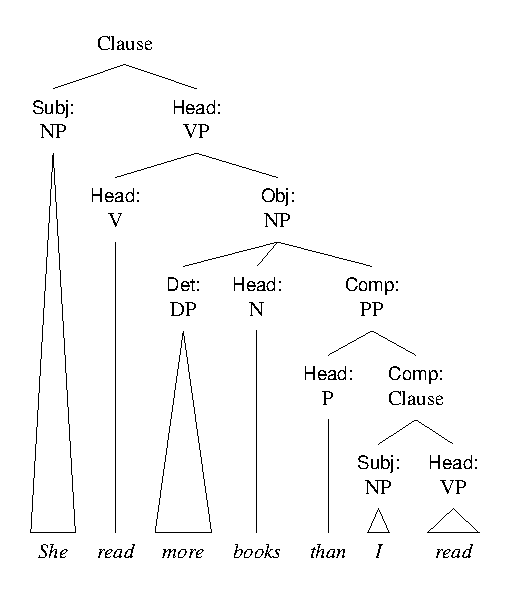
\includegraphics[width=0.7\linewidth]{figures/she read more books than I read.pdf}
    \caption{Punong sintaktiko ng sugnay-pahambing na may ellipsis}\label{fig:comp-tree-tl}
\end{figure}

Ayon sa uri ng paghahambing, gumaganap ang sugnay-pahambing bilang komplemento sa loob ng PP na may \mention{than} o \mention{as}.

\ea \label{ex:comp-markers-tl}
    \ea \gll Kim is taller than {\ob}Pat is{\cb}.\\
        Kim ay-PRS mas-matangkad than Pat ay-PRS\\
    \glt \trans{Mas matangkad si Kim kaysa kay Pat.} [hindi pagkakapantay]
    \ex \gll Kim is as tall as {\ob}Pat is{\cb}.\\
        Kim ay-PRS as matangkad as Pat ay-PRS\\
    \glt \trans{Kasingtangkad ni Pat si Kim.} [pagkakapantay\footnote{Maaaring makalito ang salitang \enquote{\term{pagkakapantay}} dito. Ang kahulugan ng halimbawang ito ay hindi mas mababa si Kim kay Pat sa tangkad; maaari ring mas matangkad si Kim.}]
    \z
\z
Sa (\ref{ex:comp-markers-tl}a), nagpapakita ng hindi pagkakapantay ang \mention{than}; sa (b), minamarkahan ng \mention{as} ang pagkakapantay. Ang unang \mention{as} ay adverb. Ang \mention{as tall} ay AdjP, at sa loob nito gumaganap ang \mention{as} bilang modifier. Ang ikalawang \mention{as} ay preposition.

May ilang hirap ang mga nag-aaral ng Ingles sa mga sugnay-pahambing.
\begin{itemize}[noitemsep]
    \item Pag-alam kung ano, kailan, at gaano karaming bahagi ang maaaring iwan.
    \item Pagkilala sa magkakaibang padron ng pagkakapantay at hindi pagkakapantay.
    \item Paghawak sa masalimuot na paghahambing na may higit sa isang elementong kasangkot.
\end{itemize}

Ang mabuting balita ay regular ang mga padron ng sugnay-pahambing. Bago pumasok sa mas masalimuot na kayarian, maaaring matutuhan muna ng mga mag-aaral ang mga batayang padron gaya ng \mention{taller than} \trans{mas matangkad kaysa ...} at \mention{as tall as} \trans{kasingtangkad ng ..., o hindi mas mababa sa tangkad kaysa ...}.

\section{Koordinasyon}\label{sec:coordination-tl}

Gumagawa ang pagpapailalim ng relasyon ng pag-asa sa pagitan ng mga sugnay; iniuugnay naman ng \term{koordinasyon} ang mga elementong may parehong sintaktikong katayuan. Nasa sentro ng sistemang ito ang isang maliit na closed word class: ang \term{pangkoordina} (\term{coordinator}, Crd). Ang pangunahing kasapi ay \mention{and}, \mention{or}, at \mention{but}; tatlo ang kailangan upang mabilang ang tatlo. Gaya ng pangpailalim, gumaganap din bilang pananda ang pangkoordina.

Dito, ang \term{koordinasyon} ay hindi lamang \enquote{magkasundo} o \enquote{may koordinasyon} sa pang-organisasyong kahulugan. Sa Tagalog, ang \enquote{koordinasyon} ay madaling maunawaan bilang pag-aayos ng gawain ng mga tao o opisina. Sa kabanatang ito, teknikal ang kahulugan: dalawa o higit pang elemento ang nasa parehong sintaktikong katayuan, at walang isa sa kanila ang ulo ng buong kayarian. Kung hindi ito malinaw, madaling mapagkamalan ang koordinasyon bilang simpleng pagdudugtong ng ideya o listahan lamang.

Tingnan ang mga sumusunod na halimbawa.

\ea \label{ex:coord-basic-tl}
    \ea \gll {\ob}Jane is a good teacher{\cb} {\ob}and her students really like her{\cb}.\\
        Jane ay-PRS a mahusay guro and her estudyante-PL talaga gusto-PRS her\\
    \glt \trans{Mahusay na guro si Jane at talagang gusto siya ng kanyang mga estudyante.}
    \ex \gll They offered us a choice of {\ob}red wine{\cb}, {\ob}white wine{\cb}, {\ob}or beer{\cb}.\\
        sila nag-alok-PST amin a pagpipilian of pula alak puti alak or serbesa\\
    \glt \trans{Inalok nila kami ng pagpipilian: pulang alak, puting alak, o serbesa.}
    \ex \gll Her assistant is {\ob}very young{\cb} {\ob}but a quick learner{\cb}.\\
        her katulong ay-PRS napaka bata but a mabilis matuto\\
    \glt \trans{Napakabata ng kanyang katulong, ngunit mabilis matuto.}
    \z
\z
Sa mga halimbawang ito, gumaganap bilang \term{elementong coordinate} (\term{coordinate}) ang mga kaugnay na bahagi. Maaaring maisagawa ang gawaing ito ng mga sugnay gaya ng (\ref{ex:coord-basic-tl}a), ng NP o iba pang parirala gaya ng (b), at mas bihira, ng pinaghalong kategorya gaya ng AdjP at NP sa (c). Karaniwang nagpapahayag ang mga pangkoordina ng tiyak na relasyon: dagdag para sa \mention{and}, pagpipilian para sa \mention{or}, at pagsalungat para sa \mention{but}.

Ang malaking kaibahan ng koordinasyon sa naunang mga kayarian ay wala itong ulo. Walang elementong coordinate na ulo ng buong kayarian. Makikita ito sa isang payak na pagsusuri. Sa maraming kaso, maaaring palitan ang buong koordinadong kayarian ng isa sa mga elementong coordinate.

\ea \label{ex:coord-replace-tl}
    \ea \gll Her assistant is very young.\\
        her katulong ay-PRS napaka bata\\
    \glt \trans{Napakabata ng kanyang katulong.}
    \ex \gll Her assistant is a quick learner.\\
        her katulong ay-PRS a mabilis matuto\\
    \glt \trans{Mabilis matuto ang kanyang katulong.}
    \z
\z
Ang (\ref{ex:coord-replace-tl}a) at (b) ay parehong gramatikal na kapalit ng (\ref{ex:coord-basic-tl}c). Iba ito sa kayariang may ulo gaya ng \mention{very young}. Sa ganoong kaso, maaaring gamitin nang mag-isa ang ulo (\mention{she's young}), ngunit hindi ang nakaasang bahagi (*\mention{she's very}). Makikita ang kayarian ng koordinasyon sa Figure~\ref{fig:coord-basic-tl}.

\begin{figure}
    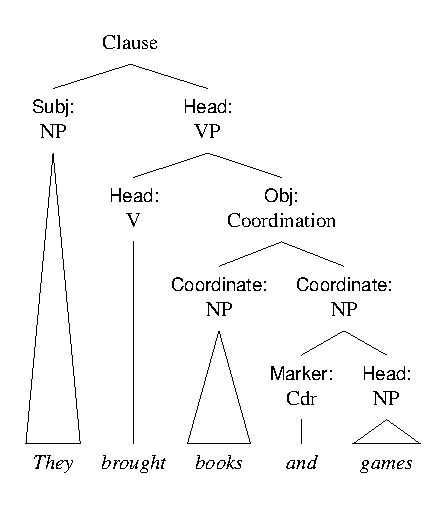
\includegraphics[width=0.65\linewidth]{figures/the brought books and games.pdf}
    \caption{Batayang koordinasyon na may pananda: \mention{They brought books and games}}\label{fig:coord-basic-tl}
\end{figure}

\subsection{Mga katangian ng koordinasyon}

May tatlong mahalagang katangian na naghihiwalay sa koordinasyon mula sa ibang kayarian.

Walang gramatikal na hangganan sa bilang ng mga elementong coordinate. Eksepsiyon ang \mention{but}.

\ea \label{ex:coord-multiple-tl}
\gll Nothing noble, sublime, profound, delicate, tasteful or even decent can find a place.\\
    wala marangal mataas malalim pino may-panlasa or kahit disente maaaring makahanap a lugar\\
\glt \trans{Walang marangal, mataas, malalim, pino, may panlasa, o kahit disente ang makakahanap ng lugar.}
\z

Dapat magkatugma ang gawain ng mga elementong coordinate. Kung gagamitin nang mag-isa, dapat kaya nilang gumanap sa parehong tungkulin.

\ea \label{ex:coordinate-function-tl}
    \ea \gll I'll be back next week or at the end of the month.\\
        ako-FUT babalik susunod linggo or at DEF dulo of DEF buwan\\
    \glt \trans{Babalik ako sa susunod na linggo o sa katapusan ng buwan.} [modipikador ng panahon]
    \ex \gll *We're leaving Rome and next week.\\
        *kami-PRS aalis Rome and susunod linggo\\
    \glt \trans{Inaasahang kayarian: aalis kami sa Roma at sa susunod na linggo. Kakaiba ito sa Ingles dahil object ang \mention{Rome}, ngunit adjunct ang \mention{next week}.} [*; object at adjunct]
    \z
\z

Hindi maaaring ilipat sa unahan ang pinalawak na elementong coordinate, ibig sabihin ang elementong coordinate na kasama ang pangkoordina.

\ea \label{ex:coord-front-tl}
    \ea \gll They attended but they aren't members.\\
        sila dumalo-PST but sila NEG-ay-PRS kasapi-PL\\
    \glt \trans{Dumalo sila, ngunit hindi sila mga kasapi.}
    \ex \gll *But they aren't members, they attended.\\
        *but sila NEG-ay-PRS kasapi-PL sila dumalo-PST\\
    \glt \trans{Inaasahang kahulugan: dumalo sila, ngunit hindi sila mga kasapi. Sa Ingles, hindi maaaring iuna sa ganitong paraan ang pinalawak na elementong coordinate na may \mention{but}.} [*]
    \z
\z

\subsection{Tungkol sa pangkoordina sa simula ng pangungusap}

May preskriptibong payo na hindi dapat simulan ang pangungusap sa pangkoordina gaya ng \mention{and} o \mention{but}. Ngunit hindi nakabatay sa gramatika o aktuwal na gamit ng Ingles ang pagbabawal na ito. Sa buong kasaysayan ng Ingles, ginagamit ng mahuhusay na manunulat ang pangkoordina sa simula ng pangungusap. Makakakita rin ng maraming halimbawa sa kabanatang ito at sa iba pang kabanata ng aklat.

Gayunman, ang pangkoordina sa simula ng pangungusap ay hindi maaaring magtali sa bagong pangungusap sa naunang pangungusap bilang koordinasyon sa makitid na sintaktikong kahulugan. Tandaan ang limitasyon sa fronting sa (\ref{ex:coord-front-tl}). Sa halip, gumaganap ito bilang \term{pang-ugnay sa diskurso} (\term{discourse connector}), na nagpapakita kung paano kaugnay ng naunang pahayag ang bagong pangungusap.

Madaling magkamali ang mambabasang Tagalog dito. Sa Tagalog, napakanatural magsimula ng pangungusap sa \enquote{at}, \enquote{pero}, \enquote{ngunit}, \enquote{subalit}, o \enquote{kaya} bilang pang-ugnay sa diskurso. Ngunit ang koordinasyon sa kabanatang ito ay ugnayang sintaktiko sa loob ng isang kayarian, kung saan magkakapantay ang mga elementong pinag-uugnay.

Estilistiko lamang ang tunay na limitasyon: kapag sobra ang pang-ugnay sa simula ng pangungusap, nagiging paulit-ulit ang estilo; kapag maingat ang gamit, tinutulungan nito ang daloy ng diskurso.

\subsection{Mga uri ng koordinasyon}

Ang pinakapayak na pagkakaiba ay sa pagitan ng \term{simetrikong koordinasyon} (\term{symmetric coordination}) at \term{asimetrikong koordinasyon} (\term{asymmetric coordination}). Sa simetrikong koordinasyon, hindi nagbabago ang kahulugan kapag pinagpalit ang ayos ng mga elementong coordinate; sa asimetrikong koordinasyon, nagbabago ito.

\ea \label{ex:coord-sym-tl}
    \ea \gll I was hungry and tired.\\
        ako naging-PST gutom and pagod\\
    \glt \trans{Gutom at pagod ako.} [simetriko]
    \ex \gll I got up and had breakfast.\\
        ako bumangon-PST and kumain-PST almusal\\
    \glt \trans{Bumangon ako at nag-almusal.} [asimetriko]
    \z
\z
Sa (\ref{ex:coord-sym-tl}a), hindi nagbabago ang kahulugan kapag pinagpalit ang ayos ng mga elementong coordinate. Ngunit sa (b), nagpapakita ng pagkakasunod sa panahon ang ayos. Nauna ang pagbangon bago ang almusal.

Ibinubukod din ang \term{distributibong koordinasyon} (\term{distributive coordination}) at \term{sama-samang koordinasyon} (\term{joint coordination}).

\ea \label{ex:coord-dist-tl}
    \ea \gll Kim and Pat are fine players.\\
        Kim and Pat ay-PRS mahusay manlalaro-PL\\
    \glt \trans{Mahuhusay na manlalaro sina Kim at Pat.} [distributibo]
    \ex \gll Kim and Pat are a good pair.\\
        Kim and Pat ay-PRS a mahusay pares\\
    \glt \trans{Magandang pares sina Kim at Pat.} [sama-sama]
    \z
\z
Sa (\ref{ex:coord-dist-tl}a), hiwalay na naaangkop kina Kim at Pat ang pagiging mahusay na manlalaro. Sa (b), totoo lamang ang pagiging magandang pares kung magkakasama silang dalawa. Hindi maaaring maging pares ang isang tao nang mag-isa.

\subsection{Pagmamarka ng koordinasyon}

Maaaring markahan ang koordinasyon sa ilang paraan.
\begin{itemize}[noitemsep]
    \item gamit ang pangkoordina: \mention{red and blue}
    \item walang tahasang pananda: \mention{red, white, blue}
    \item inuulit ang pangkoordina: \mention{red or white or blue}
    \item gamit ang magkatambal na pananda: \mention{both red and blue}
\end{itemize}

Karaniwang nagpapahayag ang pangkoordina ng dagdag (\mention{and}), pagpipilian (\mention{or}), at pagsalungat (\mention{but}); ngunit sa asimetrikong koordinasyon, maaari itong magdala ng karagdagang kahulugan.

\ea \label{ex:coord-meaning-tl}
    \ea \gll Pay within a week and you'll get a discount.\\
        magbayad within a linggo and ikaw-FUT makakuha a diskuwento\\
    \glt \trans{Kung magbabayad ka sa loob ng isang linggo, makakakuha ka ng diskuwento.} [kondisyon]
    \ex \gll Pay within a week or you'll lose the discount.\\
        magbayad within a linggo or ikaw-FUT mawala DEF diskuwento\\
    \glt \trans{Kung hindi ka magbabayad sa loob ng isang linggo, mawawala ang diskuwento.} [negatibong kondisyon]
    \z
\z

\begin{tblsframedsymbol}{Kilalanin ang padron: koordinasyon ba o pagpapailalim?}{test}
Gamitin ang mga pagsusuring diagnostiko upang paghiwalayin ang mga kayarian.
\begin{itemize}[noitemsep, leftmargin=*]
    \item Sa \mention{She thinks that he left} at \mention{She left and he stayed}: alin ang naglalagay ng isang sugnay sa loob ng isa pa, at alin ang nag-uugnay ng dalawang sugnay na magkasing-antas?
    \item Sa \mention{Although it rained, we went} at \mention{It rained but we went}: alin ang nagpapakita ng hirarkiyang pag-asa, at alin ang nagpapakita ng pagkakapantay?
    \item Sa \mention{*But we went, it rained} at \mention{Although it rained, we went}: ano ang ipinapakita nito tungkol sa fronting?
\end{itemize}
Tumutulong ang mga pagsusuring ito upang paghiwalayin ang may-patong na pagsingit at ang pag-uugnay ng mga elementong magkasing-antas.
\end{tblsframedsymbol}

Kapag naipakilala na ang pangkoordina, nakita na natin ang lahat ng pangunahing lexical category sa Ingles maliban sa interjection. Nakita rin natin ang pangunahing sintaktikong gawain nila sa loob ng sugnay.

\subsection{Kayarian ng koordinasyon}

Kapag kinokoordina ang mga elemento, kailangang magbahagi sila ng parehong sintaktikong gawain. Ibig sabihin, maaaring ikoordina ang komplemento sa komplemento, at ang modipikador sa modipikador; ngunit hindi maaaring ikoordina ang komplemento at modipikador sa isa't isa. Ihambing ang mga sumusunod.

\ea \label{ex:coord-function-tl}
    \ea \gll We listened {\ob}to the teacher{\cb} {\ob}and the students{\cb}.\\
        kami nakinig-PST to DEF guro and DEF estudyante-PL\\
    \glt \trans{Nakinig kami sa guro at sa mga estudyante.} [komplemento]
    \ex \gll We listened {\ob}Monday{\cb} and {\ob}Tuesday{\cb}.\\
        kami nakinig-PST Lunes and Martes\\
    \glt \trans{Nakinig kami noong Lunes at Martes.} [modipikador]
    \ex \gll *We listened {\ob}to the teachers{\cb} and {\ob}Monday{\cb}.\\
        *kami nakinig-PST to DEF guro-PL and Lunes\\
    \glt \trans{Kakaiba ang inaasahang kayarian sa Ingles. Komplemento ang \mention{to the teachers}, ngunit modipikador ang \mention{Monday}.} [*; magkahalong gawain]
    \z
\z
Ang mga elementong kinokoordina, o \term{elementong coordinate}, ay maaaring lumitaw sa alinmang pangunahing uri ng parirala: noun, verb, adjective, preposition, mas malaking parirala, o sugnay. Ang mahalaga ay pareho ang kanilang gawain sa loob ng mas malaking kayarian.

\subsection{Minarkahan at di-minarkahang koordinasyon}

Maaaring may tahasang pangkoordina ang koordinasyon, o maaari ring wala. Kapag walang pangkoordina, tinatawag itong \term{koordinasyong walang pangkoordina} (\term{asyndetic coordination}).

\ea \label{ex:coord-marking-tl}
    \ea \gll She brought {\ob}games{\cb}, {\ob}stories{\cb}, {\ob}songs{\cb}.\\
        siya nagdala-PST laro-PL kuwento-PL awit-PL\\
    \glt \trans{Nagdala siya ng mga laro, kuwento, at awit.} [walang pangkoordina]
    \ex \gll She brought {\ob}games{\cb}, {\ob}stories{\cb}, and {\ob}songs{\cb}.\\
        siya nagdala-PST laro-PL kuwento-PL and awit-PL\\
    \glt \trans{Nagdala siya ng mga laro, kuwento, at awit.} [may pangkoordina]
    \z
\z
Bukod sa payak na koordinasyong may isang pangkoordina, may \term{koordinasyong korelatibo} (\term{correlative coordination}). Dito, lumilitaw ang mga pananda sa higit sa isang elementong coordinate.

\ea \label{ex:coord-correlative-tl}
    \ea \gll {\ob}Both{\cb} tired {\ob}and{\cb} hungry\\
        both pagod and gutom\\
    \glt \trans{parehong pagod at gutom}
    \ex \gll {\ob}Either{\cb} now {\ob}or{\cb} never\\
        either ngayon or kailanman-hindi\\
    \glt \trans{ngayon, o hindi na kailanman}
    \ex \gll {\ob}Neither{\cb} simple {\ob}nor{\cb} easy\\
        neither simple nor madali\\
    \glt \trans{hindi simple at hindi rin madali}
    \z
\z

\subsection{May-patong na koordinasyon}

Maaaring maglaman mismo ng koordinasyon ang elementong coordinate. Matatawag itong may-patong na koordinasyon. Isaalang-alang ang sumusunod.

\ea \label{ex:coord-layered-tl}
\gll The story was {\ob}short and sweet{\cb} but {\ob}complex and thought-provoking{\cb}.\\
    DEF kuwento ay-PST maikli and matamis but masalimuot and nakapag-iisip\\
\glt \trans{Maikli at kaaya-aya ang kuwento, ngunit masalimuot at nakapag-iisip.}
\z
Dito, may dalawang pangunahing elementong coordinate na pinag-uugnay ng \mention{but}. Ngunit ang bawat isa ay may sarili ring koordinasyong may \mention{and}. Nagbibigay ang ganitong pagpapatong ng paraan upang ipahayag ang masalimuot na relasyon ng mga ideya habang malinaw pa rin ang kayarian. Makikita ang may-patong na kayarian sa Figure~\ref{fig:coord-layered-tl}.

\begin{figure}
    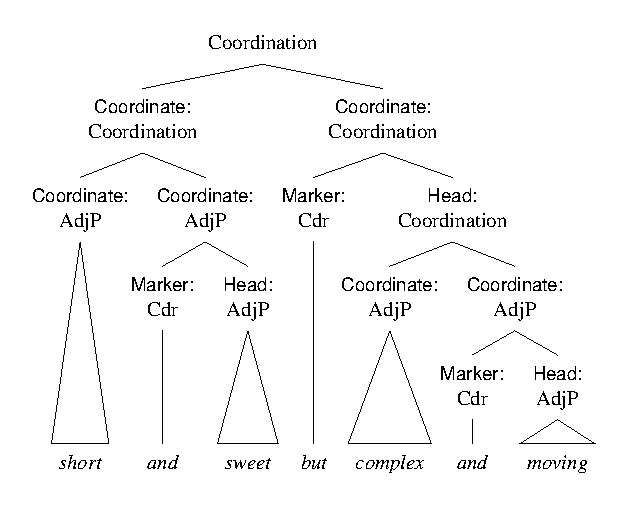
\includegraphics[width=0.9\linewidth]{figures/short and sweet but complex and moving.pdf}
    \caption{May-patong na koordinasyon: \mention{short and sweet but complex and moving}}\label{fig:coord-layered-tl}
\end{figure}

\subsection{Espesyal na koordinasyon}

May isang espesyal na kawili-wiling koordinasyon sa mga kayariang pahambing.

\ea \label{ex:coord-comp-tl}
    \ea \gll He's as tall as {\ob}or taller than{\cb} his brother.\\
        siya-ay as matangkad as or mas-matangkad than his kapatid\\
    \glt \trans{Kasingtangkad siya ng kanyang kapatid, o mas matangkad pa.}
    \ex \gll She writes more {\ob}but understands less{\cb} than before.\\
        siya sumulat-PRS mas-marami but umunawa-PRS mas-kaunti than dati\\
    \glt \trans{Mas marami siyang isinusulat kaysa dati, ngunit mas kaunti ang nauunawaan.}
    \z
\z
Sa ganitong mga kayarian, madalas na masalimuot ang relasyon ng mga elementong coordinate at ng bahaging pinaghahatian nila. Upang maipaliwanag ang mga ito, kailangang maunawaan kapwa ang koordinasyon at ang relasyong pahambing.

\begin{tblsframedsymbol}{Mabilis na sariling pagsusuri: masalimuot na kayarian}{test}
Tingnan kung kaya mong suriin ang mga may-patong na kayarian.
\begin{itemize}[noitemsep, leftmargin=*]
    \item Sa \mention{I know that she left and he stayed}, hanapin ang lahat ng relasyon ng pagpapailalim at koordinasyon.
    \item Sa \mention{Both young and talented, she succeeded}, hanapin ang magkatambal na pananda at ang mga adjective na kinokoordina.
    \item Suriin ang kayariang ito: \mention{He's taller than I thought but shorter than his brother}.
\end{itemize}
Kapag nauunawaan ang mga masalimuot na padron, makikita kung paano magkasamang lumilikha ng kahulugan ang pagpapailalim at koordinasyon.
\end{tblsframedsymbol}

\section{Buod}

Parehong nag-uugnay ng mga ideya ang pagpapailalim at koordinasyon, ngunit magkasalungat ang kayariang ginagamit nila. Nagpapasok sa loob ang pagpapailalim; nagtatambal ang koordinasyon. Binabalanse ng mahusay na pagsulat ang dalawa. Kapag naiintindihan natin kung anong kayarian ang sinusubukang buuin ng mag-aaral, at kung saan nasisira ang kayarian, hindi tayo titigil sa pagsasabing \enquote{may kakaiba}; mabibigyan natin ng pangalan ang problema. Sobra ang pagpapatong, sobra ang paglista, o gumamit ng pangpailalim kung saan sapat na ang pangkoordina--sa ganitong paraan.
